\documentclass{standalone}
\usepackage{tikz}
\usetikzlibrary{hobby, calc, intersections, spy, patterns}

\usepackage{pgfplots}
\usetikzlibrary{intersections, pgfplots.fillbetween}
% \pgfplotsset{compat=1.11}
% \usepgfplotslibrary{fillbetween}

\tikzset{%
  mark coordinate/.style={inner sep=0pt,outer sep=0pt,minimum size=1.2pt,
    fill=black,circle}%
}

\tikzset{%
  dots/.style args={#1per #2}{%
    line cap=round,
    dash pattern=on 0 off #2/#1
  }
}


% \pgfdeclarelayer{bg}
% \pgfsetlayers{bg,main}


\begin{document}
  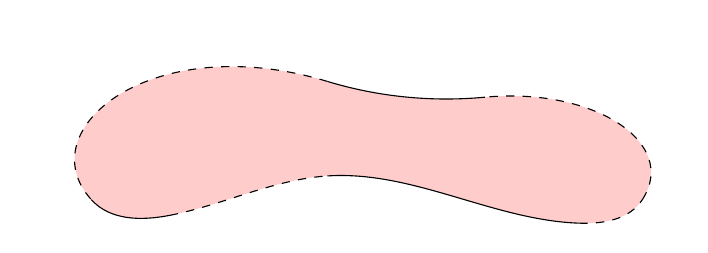
\begin{tikzpicture}[use Hobby shortcut]
    \begin{scope}[rotate=90]
      \fill[red!20!white, closed=true] (6.5,-1) .. (7.8,1) .. (8,3) .. (6.5,6) .. (6.3,5) .. (6.8,3) .. (6.2,-.2);
      \draw[closed=true] ([blank=soft]6.5,-1) .. ([blank=soft]7.8,1) .. (8,3) .. ([blank=soft]6.5,6) .. (6.3,5) .. ([blank=soft]6.8,3) .. (6.2,-.2);
      \draw[dashed, use previous Hobby path={invert soft blanks, disjoint}];
    \end{scope}
  \end{tikzpicture}
\end{document}
